\section{Entry criteria}
In order to start an integration test, two constraints must be satisfied:
the major classes must be covered by, at least, 60 percent of unit tests, 
while for the others a value of 30 percent is sufficient.
%TODO spiegare meglio quali siano le classi 'major'
%Ogni classe deve avere una percentuale di unit test del 60% per le classi principali,
%e il 30% per quelle derivate.

\section{Elements to be integrated}
In our document, ``element'' is used as synonym of ``class'';
the following list describes the classes that need to undergo an integration test, 
in order to be sure that our application will behave correctly.

\vspace{5mm}
\begin{tabular*}{1.21\textwidth}{ l p{7cm}}
 \textbf{Integration Test}: Ridesmanager	&  \\
 \hline
  Ridesmanager $\rightarrow$ Ride, Sharedride & in order to store information about the actived rides \\  
 \hline
 Ridesmanager $\rightarrow$ Taxiqueue & in order to take information of available taxis  in case of taxi request. \\
 \hline
 Ridesmanager $\rightarrow$ Controller & in order to exchange information about user's( and also guest's) requests\\
 \hline
 \end{tabular*}\\

\vspace{5mm}
\begin{tabular*}{1.21\textwidth}{ l p{7cm}}
\textbf{Integration Test}: Controller		&  \\
\hline
 Controller $\rightarrow$ User &  in order to create an ad-hoc Controller and to retrieve information about users \\  
 \hline
 Controller $\rightarrow$ Servernetworkinterface &  in order to communicate with the corresponding client side\\
 \hline
 \end{tabular*}\\

\vspace{5mm}
\begin{tabular*}{1.21\textwidth}{ l p{7cm}}
\textbf{Integration Test}: Servernetworkinterface		&  \\
 \hline
 Servernetworkinterface $\rightarrow$ Clientmessage &  in order to read client's messages \\  
 \hline
 Servernetworkinterface $\rightarrow$ Servermessage &  in order to send messages to the client\\
 \hline
\end{tabular*}\\

\vspace{5mm} 
\begin{tabular*}{1.21\textwidth}{ l p{7cm}}
 \textbf{Integration Test}: Activity	&  \\
 \hline
 Activity $\rightarrow$ Action &  in order to provides the allowed actions \\  
 \hline
 Activity $\rightarrow$ Userinterface & in order to provide the set of items this class needs to show\\
 \hline
 \end{tabular*}\\

\vspace{5mm}
 \begin{tabular*}{1.21\textwidth}{ l p{7cm}}
 \textbf{Integration Test}: Action		&  \\
 \hline
 Action $\rightarrow$ Clientnetworkinterface &  in order to send requests to the server \\    
 \hline
\end{tabular*}\\

\vspace{5mm}
 \begin{tabular*}{1.21\textwidth}{ l p{7cm}}
 \textbf{Integration Test}: Userinterface		&  \\
 \hline
 Userinterface $\rightarrow$ Clientnetworkinterface &  in order to show the right Activity according to the server message \\    
 \hline
\end{tabular*}\\

\vspace{5mm}
\begin{tabular*}{1.21\textwidth}{ l p{7cm}}
\textbf{Integration Test}: Clientnetworkinterface	&  \\
 \hline
 Clientnetworkinterface $\rightarrow$ Clientmessage & in order to send messages to the server  \\ 
 \hline
Clientnetworkinterface $\rightarrow$ Servermessage &   in order to read server's messages\\   
 \hline
\end{tabular*}
%Ridesmanager: Sharedride, Ride, Controller:{ User, Servornetwrokinterface },
%              Taxiqueue
%Servernetworkinterface: Clientmessage, Servermessage
%Activity: Action:{Clientnetworkinterface},Userinterface 
%Clientnetworkinterface: Clientmessage, Servermessage

\section{Integration testing strategy}
In this section we will explain how we planned the integration test
in order to build, as soon as possible, a running application 
with few working features; this will allow us to promptly show
our progress to the customer and also, in case of a delay in the development, 
to launch a working application, although with missing requirements.
In order to reach our goal we decided to apply a \textit{bottom-up} method
during the integration test phase, and a \textit{top-down} one for the unit tests.\\
The first working version of our application will include major classes;
in this milestone, there are no users, but only a guest that has the possibility  % domanda: un singolo unico guest?
to access all the already implemented features.\\
The second version will add multiple other users with the related constraints,
as explained in the previous documents (see RASD and Design Document).\\
From the second version onward, the application could be released,
even if only few features are already implemented.\\
The next versions will include other features that allow us to meet  % le includeranno *gradualmente*? 
all the missing requirements.
%Unit testing->Top-down
%Integration testing->bottom-up

\section{Sequence of component/Function integration}
%1- Componenti base del server: Ridesmanager, Controller, Guestcontroller
%2- Componenti base del client: Action, LoginAction, Activity, Userinterface
%   			        ^^^^^^^^^^^^^^^^^^^^^^^^^^ rivedere questa sequenza
%3- Componenti base networking: Clientnetworkinterface Servernetworkinterface,
%                               Clientmessage, Servermessage
%4- Integrazione server-client
%5- Componenti utente: User, Taxidriver, Passenger, Passengerscontroller
%                      Taxidriverscontroller, Ride
%6- Integrazione utente
%7- Fuznioni avanzate: Sharedride, Reservation
%8- Integrazione funzioni avanzate

\subsection{Software integration sequence}
The software integration sequence is shown in Figure \ref{fig:soft_int}
\begin{figure} [h]
  \centering
  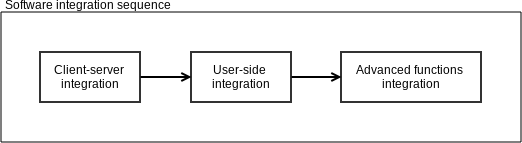
\includegraphics[scale=0.72]{diagrams/software integration.png}
  \caption{\label{fig:soft_int} Software integration}
\end{figure}
%punti: 4, 6, 8

\subsection{Subsystem integration sequence}
The classes presented in the following figures are ordered according to the sequence in which they will be tested, which is:
\ref{fig:base_serv_comp} $\rightarrow$ \ref{fig:base_client_comp} $\rightarrow$ \ref{fig:base_net_comp}
 $\rightarrow$ \ref{fig:ext_client_comp} $\rightarrow$ \ref{fig:adv_func}

Note: the arrows here represent the ordering of the integration, which may happen to partially
match the logical structure of the project; however, those arrows do not aim to describe the inter-class
relationships

% queste è meglio sistemarle bene quando la sezione precedente è consolidata
%   -- Il vate(r)
\begin{figure} [h]
  \centering
  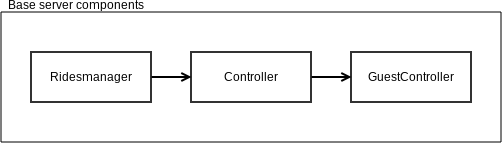
\includegraphics[scale=0.72]{diagrams/point 1.png}
  \caption{\label{fig:base_serv_comp} Base server components}
  \vspace{3mm}
  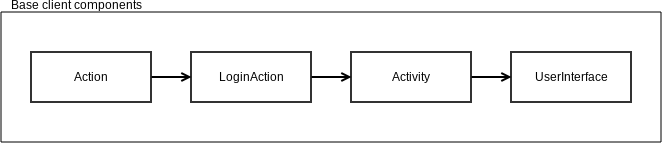
\includegraphics[scale=0.6]{diagrams/point 2.png}
  \caption{\label{fig:base_client_comp} Base client components}
  \vspace{3mm}
  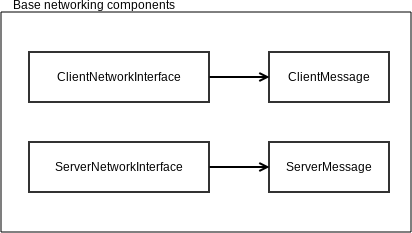
\includegraphics[scale=0.72]{diagrams/point 3.png}
  \caption{\label{fig:base_net_comp} Base networking components}
  \vspace{3mm}
  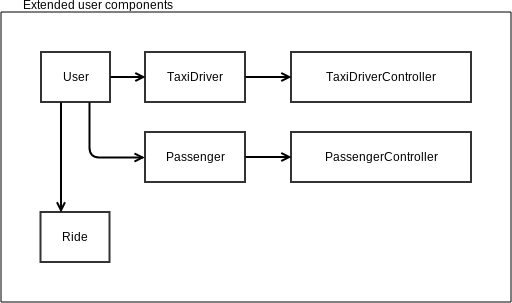
\includegraphics[scale=0.68]{diagrams/point 5.png}
  \caption{\label{fig:ext_client_comp} Extended client components}
\end{figure}
\begin{figure} [h]
  \centering
  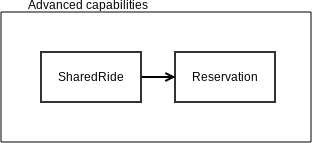
\includegraphics[scale=0.72]{diagrams/point 7.png}
  \caption{\label{fig:adv_func} Advanced functions}
\end{figure}

%punti: 1,2,3,5,7

